\section{Why is Lattice Crypto important, interesting,\ldots}
\begin{frame}{Why is Lattice Based Crypto important?}{Or interesting? Or\ldots? Buzzword Bingo.}
    \begin{block}{Some facts}
    \begin{itemize}
        \visible<1->{\item It is a Post-Quantum secure Cryptosystem (PQC)}
        \visible<2->{\item It is damn fast (faster than dinosauRS cryptA)}
        \visible<3->{\item You can build anything you want from it:\\
                  Encryption, Signatures, even Hash Functions!}
        \visible<4->{\item It allows to build even some of the most advanced cryptographic building blocks: \begin{itemize}
                     \item Fully Homomorphic Encryption (FHE),
                     \includemedia[
                     addresource=data/holygrenade.mp3,
                     flashvars={source=data/holygrenade.mp3
                                &autoplay=true}]{(The Holy Grail!)}{APlayer.swf}
                     \item Multi-linear Maps,
                     \item Identity-based Encryption (IBE),
                     \item \ldots
                     \end{itemize}
                    }
    \end{itemize}
    \end{block}
\end{frame}

\begin{frame}{Why is Lattice Based Crypto important?}{Is everything done?}
    \begin{block}{Fully Homomorphic Encryption}
        \centering
        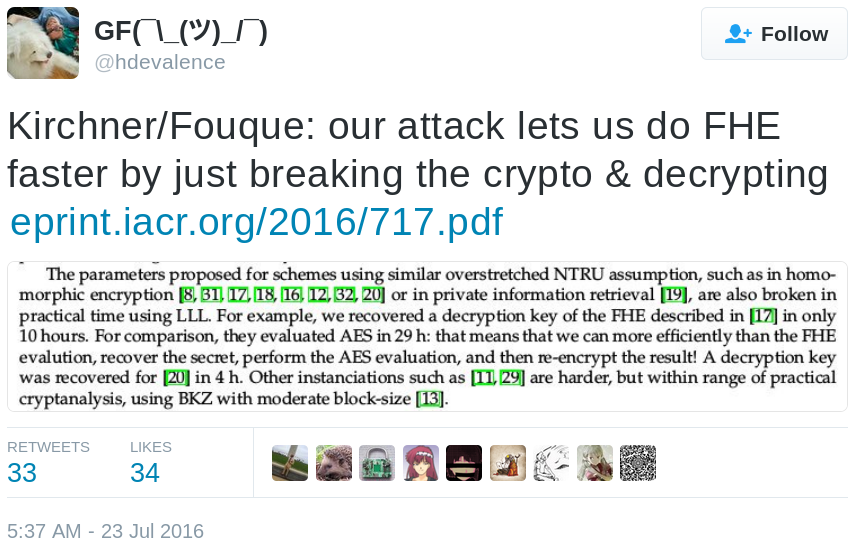
\includegraphics[keepaspectratio,height=0.75\textheight,width=\textwidth]{data/twitter_on_fhe.png}
    \end{block}
\end{frame}

\begin{frame}{The new cool kid in town.}
    \begin{block}{What is this Hype?}
    \begin{itemize}
        \visible<1->{\item \enquote{Lattice based Crypto is one of the most promising PQC candidates blablabla} (almost every paper on lattices)}
        \visible<2->{\item NSA supported this by announcing the need for PQC~\cite{riddle_enigma} in 2015}
        \visible<3->{\item Alkim~\etal/ won this year's Internet Defense Prize~\cite{idp2016} for their lattice based key exchange \enquote{New Hope}~\cite{new_hope}}
        \visible<4->{\item Google even implemented this in Chrome~\cite{google_new_hope}}
        \visible<5->{\item So, research is really vibrant here}
    \end{itemize}
    \end{block}
\end{frame}

\begin{frame}{Everything was fine.\\And then Shor entered the stage\ldots}
    \begin{columns}
        \begin{column}{0.55\textwidth}
            \begin{block}{A cryptographic thriller}
                \begin{itemize}
                    \visible<2->{%
                    \item \ldots and published an efficient CVP quantum algorithm~\cite{shor}
                    \item for one day the cryptographic community was shocked!
                    }
                    \visible<3->{%
                    \item \ldots and then Regev saved us all by finding a flaw in the paper~\cite{regev}
                    \item but still, Google stopped its PQ key exchange experiment with New Hope~\cite{google_new_hope2}
                    }
                \end{itemize}
            \end{block}
        \end{column}
        \begin{column}{0.4\textwidth}
            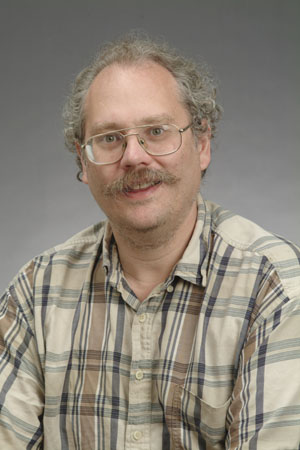
\includegraphics[keepaspectratio,height=0.75\textheight]{data/shor.jpg}
        \end{column}
    \end{columns}
\end{frame}

\begin{frame}[plain]
    \centering\Large
    Enough motivation!\\[1em]
    How does Lattice Crypto work?
\end{frame}

\section{How does Lattice Crypto work?}
\begin{frame}{How does Lattice Based Crypto work?}{Wait! Lattice, wtf?}
    \visible<1->{%
    \begin{block}{Definition:}
        A lattice $L$ is an discrete, additive, abelian subgroup of $\mathbb{R}^n$.
    \end{block}}
    \visible<2->{%
    \begin{block}{Definition:}
        Let $b_1, b_2, \ldots{}, b_d \in \mathbb{R}^n,\ d \leq n$ linear independent.
        Then the set
        \begin{equation*}
            L = \set{v \in \mathbb{R}^n \given v = \sum_{i=1}^{d} a_i b_i, a_i \in \mathbb{Z}}
        \end{equation*}
        is a lattice.
    \end{block}}
\end{frame}

\begin{frame}{Hey! You promised, this will be easy!}
    \begin{block}{Lattice, dt\@.: Gitter}
        \centering
        
\includegraphics[keepaspectratio, width=\textwidth, height=0.5\textheight]{data/gitterkartoffel.jpg}
    \end{block}
\end{frame}

\begin{frame}{Hey! You promised, this will be easy!}{OK, OK, we can say it easier: $\mathbb{Z}^2$ is a Lattice}
    \begin{columns}
        \visible<1->{%
        \begin{column}{0.4\textwidth}
            \begin{block}{\only<1>{Example lattice}\only<2->{Random Basis\vphantom{p}}}
                \centering
                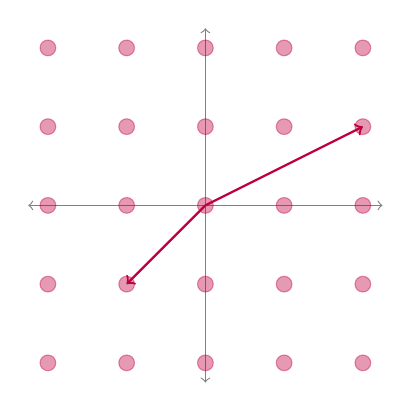
\begin{tikzpicture}
                    \draw [gray] [<->] (-2.25,0) -- (2.25,0);
                    \draw [gray] [<->] (0,-2.25) -- (0,2.25);

                    \foreach \i in {-2, -1, 0, 1, 2}{%
                        \foreach \j in {-2, -1, 0, 1, 2}{%
                            \draw [fill,purple,opacity=.4] (\i,\j) circle [radius=0.1];
                        }
                    }
                    \only<2->{%
                        \draw [thick,purple] [->] (0,0) -- (2, 1);
                        \draw [thick,purple] [->] (0,0) -- (-1, -1);
                    }
                \end{tikzpicture}
            \end{block}
        \end{column}
        }

        \visible<3->{%
        \begin{column}{0.4\textwidth}
            \begin{block}{Reduced Basis\vphantom{p}}
                \centering
                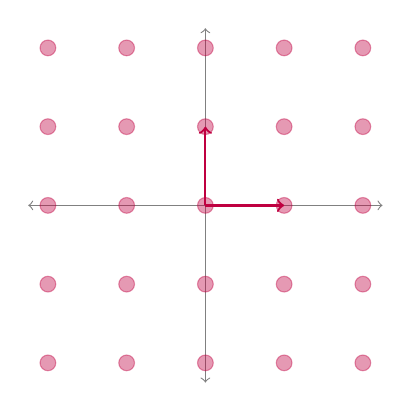
\begin{tikzpicture}
                    \draw [gray] [<->] (-2.25,0) -- (2.25,0);
                    \draw [gray] [<->] (0,-2.25) -- (0,2.25);

                    \foreach \i in {-2, -1, 0, 1, 2}{%
                        \foreach \j in {-2, -1, 0, 1, 2}{%
                            \draw [fill,purple,opacity=.4] (\i,\j) circle [radius=0.1];
                        }
                    }

                    \draw [thick,purple] [->] (0,0) -- (1, 0);
                    \draw [thick,purple] [->] (0,0) -- (0, 1);
                \end{tikzpicture}
            \end{block}
        \end{column}
        }
    \end{columns}
    {\vspace{1em}\small In general, basis reduction is a hard problem!
        The LLL and BKZ algorithm are available for this. NTL's implementation of BKZ has $2^{n^2}$ runtime.}
\end{frame}

\begin{frame}{Hard Problems in Lattices\ldots}{\ldots are what we need for crypto.}
    \begin{columns}
        \visible<1->{%
        \begin{column}{0.55\textwidth}
            \begin{block}{Shortest Vector Problem (SVP)}
                Given a lattice $L$, what is the shortest vector $v \in L\setminus \set{\mathbf{0}}$?
            \end{block}
        \end{column}
        }

        \visible<2->{%
        \begin{column}{0.4\textwidth}
            \begin{block}{Example}
                \centering
                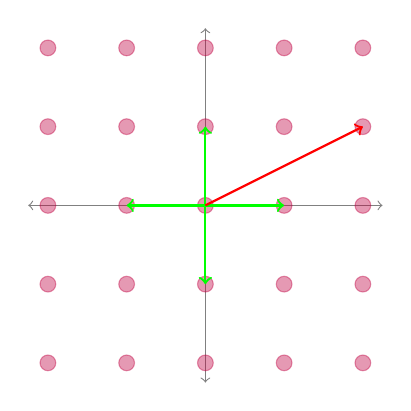
\begin{tikzpicture}
                    \draw [gray] [<->] (-2.25,0) -- (2.25,0);
                    \draw [gray] [<->] (0,-2.25) -- (0,2.25);

                    \foreach \i in {-2, -1, 0, 1, 2}{%
                        \foreach \j in {-2, -1, 0, 1, 2}{%
                            \draw [fill,purple,opacity=.4] (\i,\j) circle [radius=0.1];
                        }
                    }

                    \draw [thick,green] [->] (0,0) -- (1, 0);
                    \draw [thick,green] [->] (0,0) -- (0, 1);
                    \draw [thick,green] [->] (0,0) -- (-1, 0);
                    \draw [thick,green] [->] (0,0) -- (0, -1);
                    \draw [thick,red] [->] (0,0) -- (2, 1);
                \end{tikzpicture}
            \end{block}
        \end{column}
        }
    \end{columns}
\end{frame}

\begin{frame}{Hard Problems in Lattices\ldots}{\ldots are what we need for crypto.}
    \begin{columns}
        \visible<1->{%
        \begin{column}{0.55\textwidth}
            \begin{block}{Closest Vector Problem (CVP)}
                Given a lattice $L$ and a target $t \notin L$, what is the closest vector $v \in L$ to $t$\vphantom{$v \in L\setminus \set{\mathbf{0}}$}?
            \end{block}
        \end{column}
        }

        \visible<2->{%
        \begin{column}{0.4\textwidth}
            \begin{block}{Example}
                \centering
                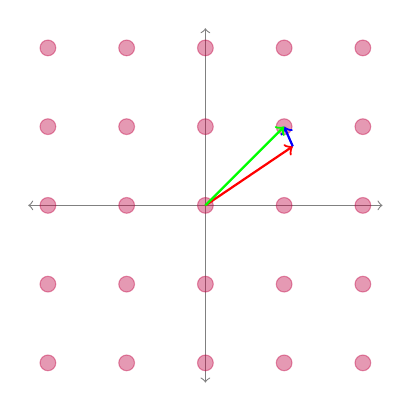
\begin{tikzpicture}
                    \draw [gray] [<->] (-2.25,0) -- (2.25,0);
                    \draw [gray] [<->] (0,-2.25) -- (0,2.25);

                    \foreach \i in {-2, -1, 0, 1, 2}{%
                        \foreach \j in {-2, -1, 0, 1, 2}{%
                            \draw [fill,purple,opacity=.4] (\i,\j) circle [radius=0.1];
                        }
                    }
                    \draw [thick,red] [->] (0,0) -- (1.11, 0.75);
                    \draw [thick,blue] [->] (1.11, 0.75) -- (1, 1);
                    \draw [thick,green] [->] (0,0) -- (1, 1);
                \end{tikzpicture}
            \end{block}
        \end{column}
        }
    \end{columns}
\end{frame}


\begin{frame}{Lattice Based Crypto}{Learning With Errors -- or: the equivalent to textbook RSA}
    \only<1>{%
    \begin{block}{Key Generation\footnote{Thanks to Elena for the nice pictures.}}
        \centering
        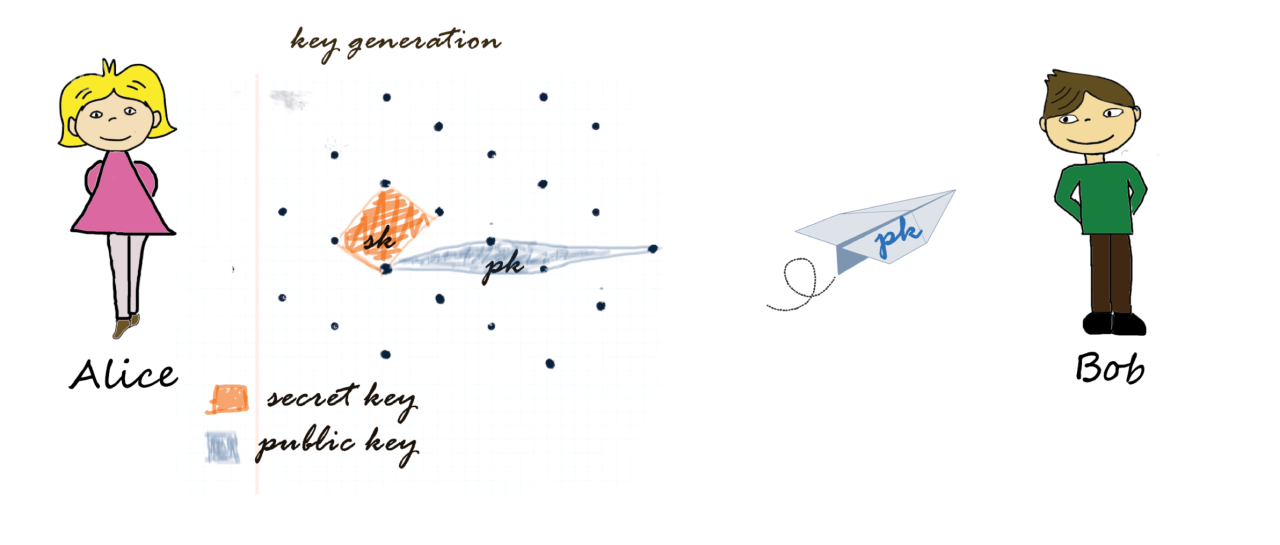
\includegraphics[keepaspectratio,width=\textwidth,height=0.8\textheight]{data/keygen}
    \end{block}
    }
    \only<2>{%
    \begin{block}{Encryption}
        \centering
        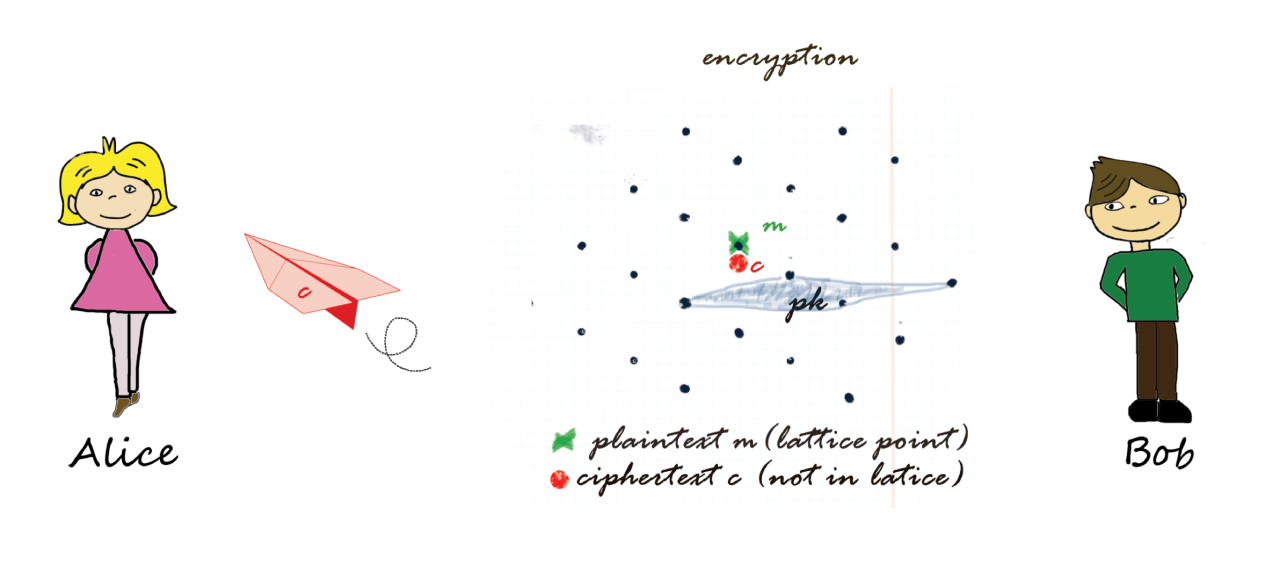
\includegraphics[keepaspectratio,width=\textwidth,height=0.8\textheight]{data/encryption}
    \end{block}
    }
    \only<3>{%
    \begin{block}{Decryption}
        \centering
        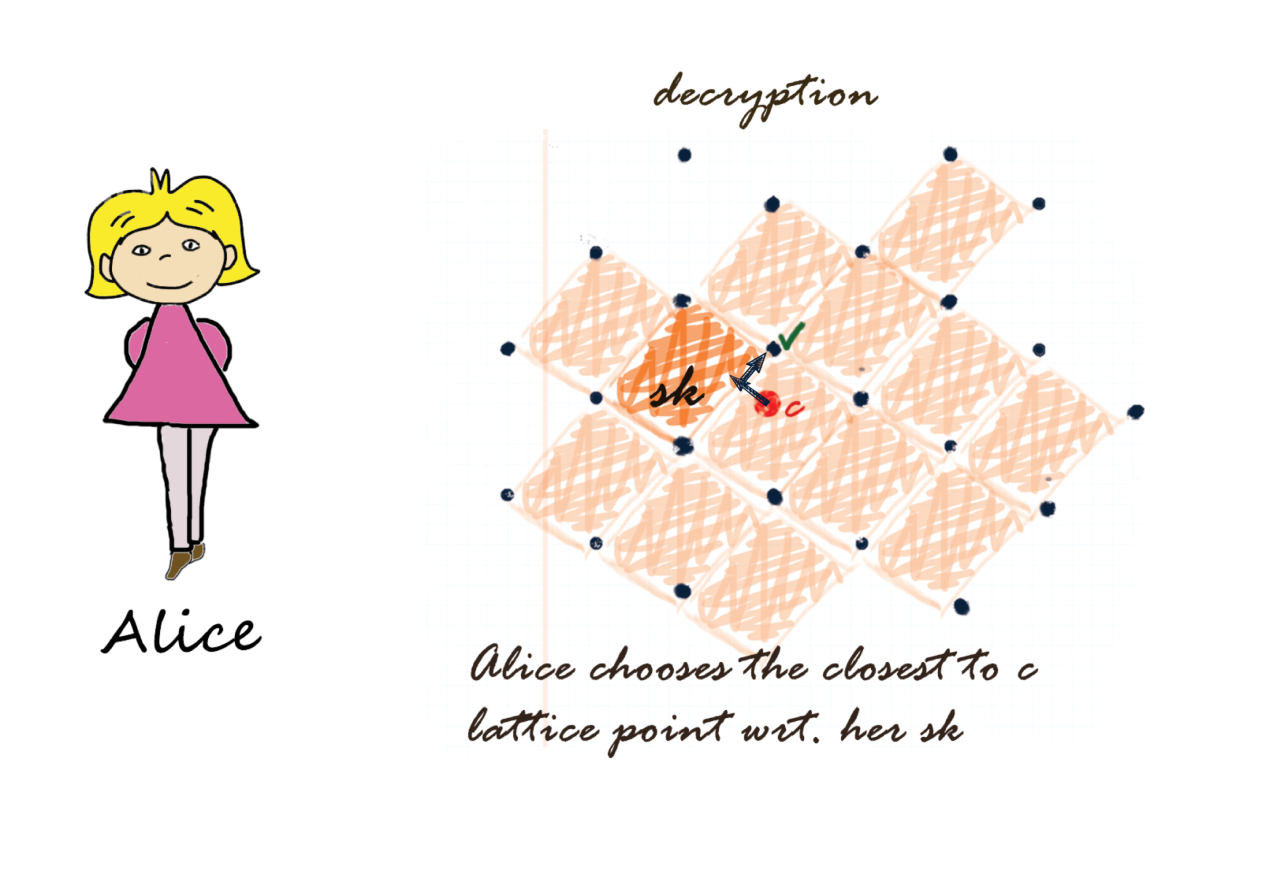
\includegraphics[keepaspectratio,width=\textwidth,height=0.8\textheight]{data/decryption}
    \end{block}
    }
\end{frame}

\section{Attacks on Lattice Based Crypto}
\begin{frame}{Attack Algorithm}
    \centering
    In practice most efficient strategy is Babai's Nearest Plane~\cite{babai},\\
    improved by Lindner and Peikert~\cite{lindner_peikert} and Gama~\etal/~\cite{gama}.
\end{frame}

\begin{frame}{Nearest Plane}{or BDD Enumeration}
    \only<1>{%
    \begin{block}{Attack}
        \centering
        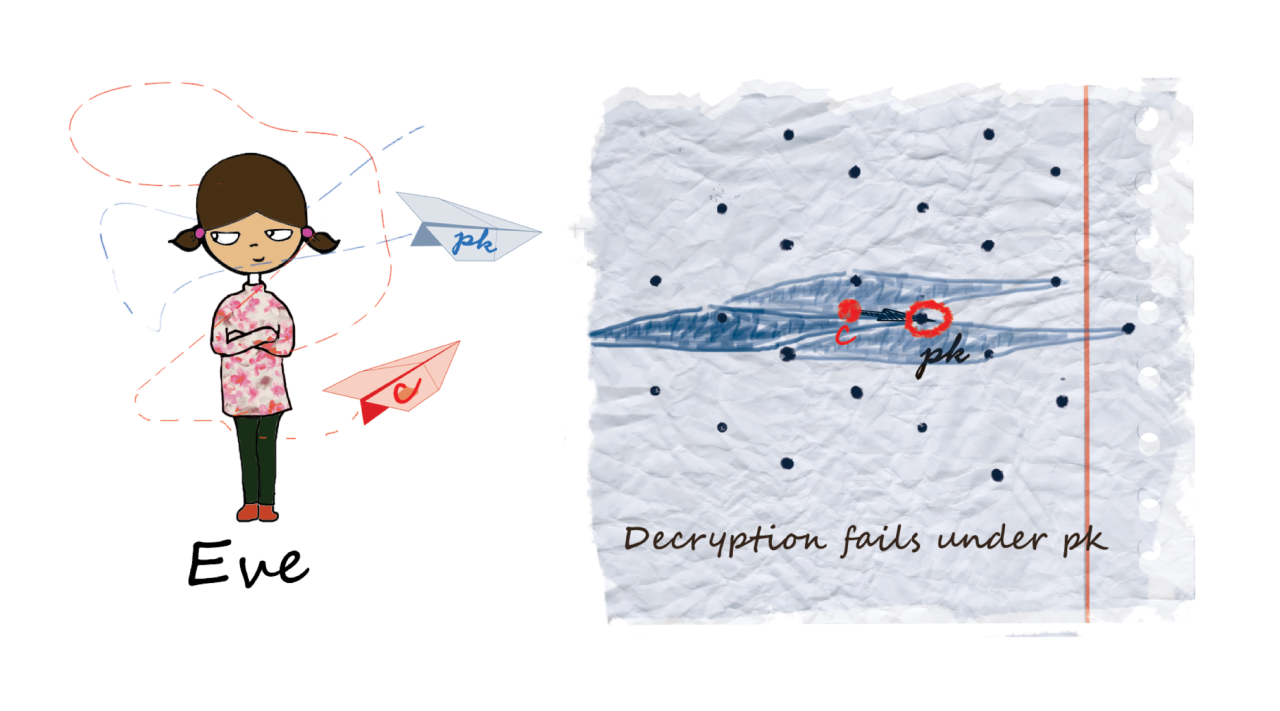
\includegraphics[keepaspectratio,width=\textwidth,height=0.8\textheight]{data/Eve}
    \end{block}
    }
    \only<2>{%
    \begin{block}{Step 1: Basis Reduction}
        \centering
        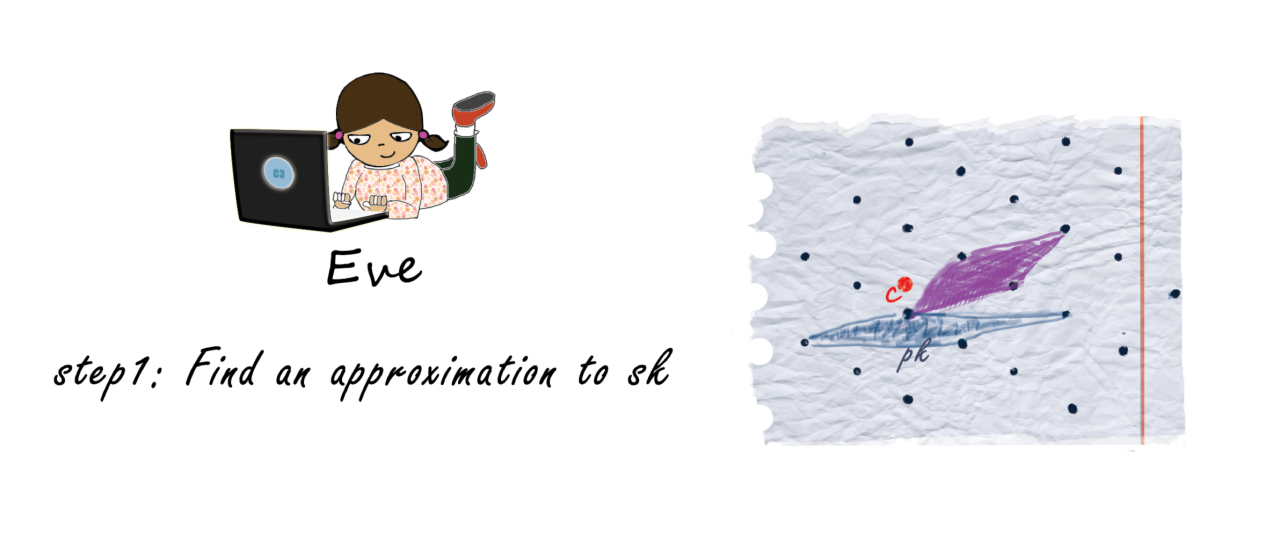
\includegraphics[keepaspectratio,width=\textwidth,height=0.8\textheight]{data/attack_step1}
    \end{block}
    }
    \only<3>{%
    \begin{block}{Step 2: Enumerate Nearest Planes}
        \centering
        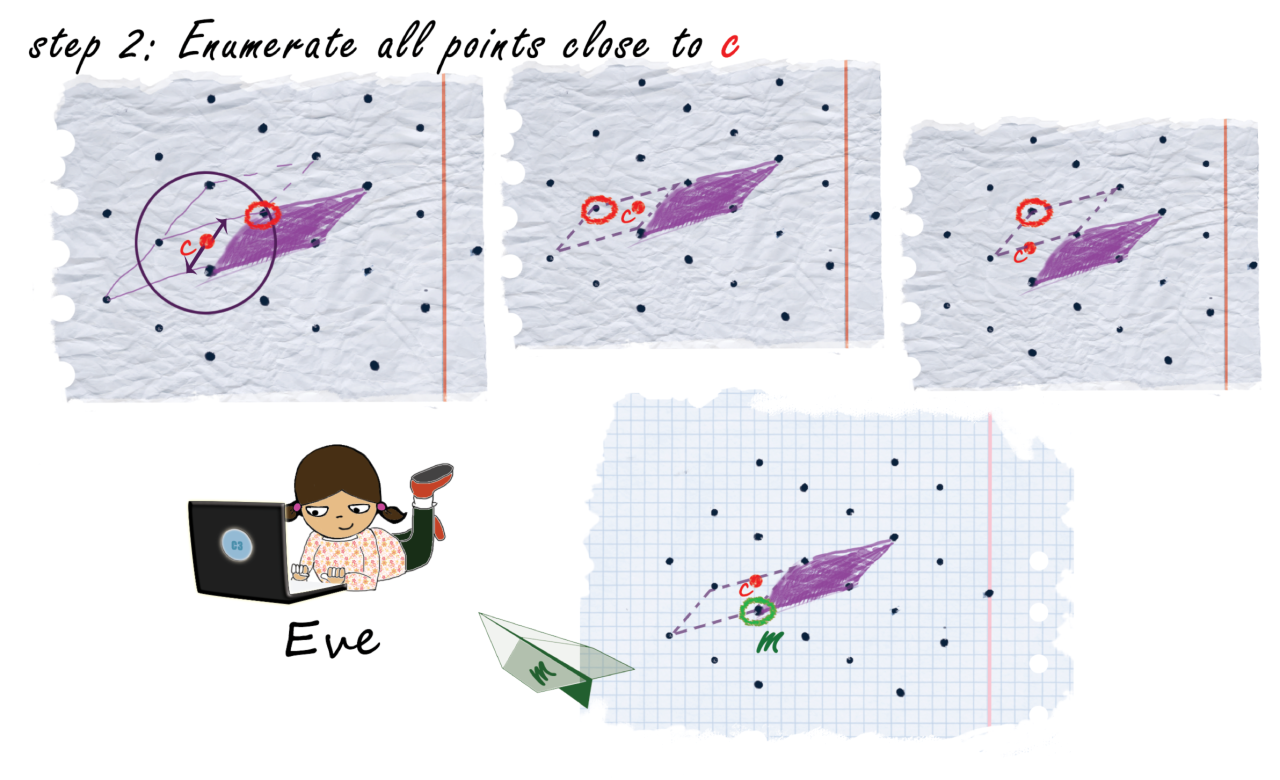
\includegraphics[keepaspectratio,width=\textwidth,height=0.8\textheight]{data/attack_step2}
    \end{block}
    }
\end{frame}

\section{OK\@. And what did I do?}
\begin{frame}{Parallel Implementation of\\BDD enumeration for LWE}
    \centering
    Finally, what we (joint work with Elena Kirshanova and Alex May) did:
    \begin{block}{Research Project}
        \begin{itemize}
            \item Goal: What is the \emph{practical} runtime of BDD enumeration?
            \item Build a parallel implementation of \texttt{NearestPlanes}.
            \item Test this on some large scale parallel system.
            \item Hopefully break some real world parameters.
        \end{itemize}
    \end{block}
\end{frame}

\begin{frame}{Parallelisation of Enumeration}{Elena's explanation}
Closest point search via depth-first tree-traversal:

\begin{center}
\begin{tikzpicture}[remember picture]
    \clip (-35pt,-30pt) rectangle (70pt, 70pt);
    \draw[step=10pt,gray,opacity=0.6, very thin] (-40pt,-30pt) grid (100pt, 100pt);
    \foreach \y in {-2,...,5}{%
        \foreach \x in {-2,...,3}{%
            \filldraw(\x*40pt+\y*10pt, 10pt*\x+20pt*\y) circle (1pt);}
    }
    \filldraw(0pt,0pt) circle (1pt) node[font=\tiny, below] {$0$};

    \draw[->, black, thin] (0,0) -- (40pt, 10pt) node[font=\tiny, below]{$b_1$};
    \draw[->, black, thin] (0,0) -- (10pt, 20pt) node[font=\tiny, below]{$b_2$};
    %\draw[->, black, very thin] (0,0) -- (-4pt, 11pt) node[font=\tiny, below]{$\bvec_2^*$};
    \filldraw[fill=red](30pt, 36pt) circle (1.5pt) node [font=\tiny, right]{$t$};

    %vertical lines:
    \draw[gray, opacity=0.4] (-40pt, -10pt) -- (0pt, 70pt);
    \draw[gray, opacity=0.4] (-20pt, -40pt) -- (40pt, 80pt);
    \draw[gray, opacity=0.4] (20pt, -30pt) -- (70pt, 70pt);
    \draw[gray, opacity=0.4] (50pt, -40pt) -- (70pt, 0pt);

    %horizontal lines:
    \draw[gray, opacity=0.4] (-50pt, 40pt) -- (70pt, 70pt);
    \draw[gray, opacity=0.4] (-60pt, 20pt) -- (100pt, 60pt);
    \draw[gray, opacity=0.4] (-70pt, 0pt) -- (90pt, 40pt);
    \draw[gray, opacity=0.4] (-40pt, -10pt) -- (80pt, 20pt);
    \draw[gray, opacity=0.4] (-50pt, -30pt) -- (70pt, 0pt);

    \visible<2->{%
    \only<2>{%
        \draw[black, thin] (32pt, 25pt) -- (30pt, 36pt) -- (25pt, 59pt);
    }

    \only<2-5>{%
        \filldraw[fill=red] (32pt, 25pt) circle (1pt) node [black, font=\tiny, below]{$t_3$};
        \filldraw[fill=red] (28.5pt, 42pt) circle (1pt) node [black, font=\tiny, right]{$t_2$};
        \filldraw[fill=red] (25pt, 59pt) circle (1pt) node [black, font=\tiny, above]{$t_1$};
    }

    \only<2>{%
        \draw [decorate,decoration={brace, amplitude=5pt}] (30pt, 36pt) -- (25pt, 59pt) node [font=\tiny, black, left, midway, yshift=-1pt, xshift=-2pt] {$\|e_1\|$};
    }

    \visible<3->{%
    \filldraw[fill=blue] (30pt, 60pt) circle (1.5pt) node{};

    \visible<4->{%
    \filldraw[fill=blue] (20pt, 40pt) circle (1.5pt) node{};

    %\pause
    \visible<5->{%
    \filldraw[fill=blue] (50pt, 30pt) circle (1.5pt) node{};
    \filldraw[fill=blue] (10pt, 20pt) circle (1.5pt) node{};
    %\pause
    \visible<6->{%
    \draw [fill=blue, opacity=0.3] (30pt, 36pt) circle (26pt);
}}}}}
\end{tikzpicture} \hspace{15pt}
\begin{tikzpicture}[level distance=1.5cm,
    level 1/.style={sibling distance=1.8cm},
    level 2/.style={sibling distance=1.2cm}]
    \node (Root) {$t$}
    child[visible on=<2->] {node {\footnotesize ($t_1, e_1$)}{%
            child[visible on=<3->] {node {\footnotesize($t_{11}, e_{11}$)}}
        }
    }
    child[visible on=<2->] {node {\footnotesize ($t_2, e_2$)}
        child[visible on=<4->] {node {\footnotesize($t_{21}, e_{21}$)}}
    }
    child [visible on=<2->]{node {\footnotesize ($t_3, e_3$)}
        child[visible on=<5->] {node {\footnotesize ($t_{31}, e_{31}$)}}
        child[visible on=<5->] {node {\footnotesize($t_{32}, e_{32}$)}}
    };

    \begin{scope}[every node/.style={right}]
        \visible<3->{%
            \path (Root-1  -| Root-3) ++(12mm,0) node {\tiny $ \|e_i\| \leq R$ };
        }
        \visible<5->{%
            \path (Root-1-1 -| Root-3-2) ++(6mm,0) node {\tiny $  \|e_j\| \leq R'$};
        }
    \end{scope}

\end{tikzpicture}
\end{center}

\visible<6->{%
    \# Leaves to visit $= 2^{n \log n}$ for $n$-dim BDD
}
\end{frame}

\begin{frame}{Results}
    After more than one year of work, two submissions and\\
    something like over 9000 weeks of benchmarking\\[1em]
    \begin{block}{We ended up with:}
        \begin{itemize}
            \visible<2->{%
            \item an open source implementation: \url{https://github.com/pfasante/cvp-enum}
            \item an ACNS paper~\cite{acns} and a Best Student Paper Award \Laughey{}
            \item huge table of runtimes
            }
        \end{itemize}
    \end{block}
\end{frame}

\begin{frame}{Results: Numbers!}
    \only<1>{%
        \begin{block}{Standard LWE}
            \begin{table}[t!]
                \centering
                \begin{tabular}{ccc|c|cc}
                    \multicolumn{3}{c|}{LWE-parameters} & {BKZ-reduction}  & \multicolumn{2}{c}{Enumeration} \\
                    $n$   & $q$    & $|e| \leq $                      & $T$             & \# Threads & $T$      \\ \midrule
                    $90$   & $4093$    & $10$                      & 11.3h            & 1 & 35h      \\
                    $90$   & $4093$    & $10$                      & 11.3h            & 10 & 3.6h \\ \midrule
                    $100$   & $4093$    & $10$                      & 7h             & 24 & 2.7h \\
                \end{tabular}
            \end{table}
        \end{block}
        \vfill{}
        To be compared with: $(n=192, |e| < 18, q=4093)$ reaches $2^{87}$-security level~\cite{lindner_peikert}.
    }
    \only<2>{%
        \begin{block}{LWE variant: Small secret}
            \begin{table}[t!]
                \begin{tabular}{ccc|c|cc}

                    \multicolumn{3}{c|}{LWE-parameters} & {BKZ-reduction}  & \multicolumn{2}{c}{Enumeration} \\
                    $n$   & $q$     & $m$     & $T$             & \# Threads & $T$      \\ \midrule
                    $140$ & $16411$     & $170$     & $12$h             & 1 & $16$h  \\
                    $140$ & $16411$     & $170$     & $12$h             & 10 & $1.7$h  \\
                \end{tabular}
            \end{table}
        \end{block}
        \vfill{}
        To be compared with: $(n=128, q=16411, m =2^{28}, T=13\text{h} )$ for combinatorial attack on LWE~\cite{BKW}.
    }
    \only<3>{%
        \begin{block}{LWE variant: Binary matrix}
            \begin{table}[t!]
                \begin{tabular}{ccc|c|c}
                    \multicolumn{3}{c|}{LWE-parameters} & {BKZ-reduction}  & {Enumeration} \\
                    $n$   & $q$     & $m$     & $T$             & $T$      \\ \midrule
                    $256$ & $500009$     & $440$     & $4.5$h             & $2$min  \\
                \end{tabular}
            \end{table}
        \end{block}
        \vfill{}
        To be compared with: Estimation by Galbraith~\cite{binary_matrix} roughly one day.
    }
\end{frame}
